\documentclass{book}
\usepackage[a4paper,top=2.5cm,bottom=2.5cm,left=2.5cm,right=2.5cm]{geometry}
\usepackage{makeidx}
\usepackage{natbib}
\usepackage{graphicx}
\usepackage{multicol}
\usepackage{float}
\usepackage{listings}
\usepackage{color}
\usepackage{ifthen}
\usepackage[table]{xcolor}
\usepackage{textcomp}
\usepackage{alltt}
\usepackage{ifpdf}
\ifpdf
\usepackage[pdftex,
            pagebackref=true,
            colorlinks=true,
            linkcolor=blue,
            unicode
           ]{hyperref}
\else
\usepackage[ps2pdf,
            pagebackref=true,
            colorlinks=true,
            linkcolor=blue,
            unicode
           ]{hyperref}
\usepackage{pspicture}
\fi
\usepackage[utf8]{inputenc}
\usepackage{mathptmx}
\usepackage[scaled=.90]{helvet}
\usepackage{courier}
\usepackage{sectsty}
\usepackage{amssymb}
\usepackage[titles]{tocloft}
\usepackage{doxygen}
\lstset{language=C++,inputencoding=utf8,basicstyle=\footnotesize,breaklines=true,breakatwhitespace=true,tabsize=4,numbers=left }
\makeindex
\setcounter{tocdepth}{3}
\renewcommand{\footrulewidth}{0.4pt}
\renewcommand{\familydefault}{\sfdefault}
\hfuzz=15pt
\setlength{\emergencystretch}{15pt}
\hbadness=750
\tolerance=750
\begin{document}
\hypersetup{pageanchor=false,citecolor=blue}
\begin{titlepage}
\vspace*{7cm}
\begin{center}
{\Large 9917144\-\_\-homework1 }\\
\vspace*{1cm}
{\large Generated by Doxygen 1.8.3.1}\\
\vspace*{0.5cm}
{\small Mon Mar 11 2013 19:23:04}\\
\end{center}
\end{titlepage}
\clearemptydoublepage
\pagenumbering{roman}
\tableofcontents
\clearemptydoublepage
\pagenumbering{arabic}
\hypersetup{pageanchor=true,citecolor=blue}
\chapter{Hierarchical Index}
\section{Class Hierarchy}
This inheritance list is sorted roughly, but not completely, alphabetically\-:\begin{DoxyCompactList}
\item Frame\-Listener\begin{DoxyCompactList}
\item \contentsline{section}{Base\-Application}{\pageref{class_base_application}}{}
\begin{DoxyCompactList}
\item \contentsline{section}{Basic\-Tutorial\-\_\-00}{\pageref{class_basic_tutorial__00}}{}
\end{DoxyCompactList}
\end{DoxyCompactList}
\item Key\-Listener\begin{DoxyCompactList}
\item \contentsline{section}{Base\-Application}{\pageref{class_base_application}}{}
\end{DoxyCompactList}
\item Mouse\-Listener\begin{DoxyCompactList}
\item \contentsline{section}{Base\-Application}{\pageref{class_base_application}}{}
\end{DoxyCompactList}
\item Sdk\-Tray\-Listener\begin{DoxyCompactList}
\item \contentsline{section}{Base\-Application}{\pageref{class_base_application}}{}
\end{DoxyCompactList}
\item Window\-Event\-Listener\begin{DoxyCompactList}
\item \contentsline{section}{Base\-Application}{\pageref{class_base_application}}{}
\end{DoxyCompactList}
\end{DoxyCompactList}

\chapter{Class Index}
\section{Class List}
Here are the classes, structs, unions and interfaces with brief descriptions\-:\begin{DoxyCompactList}
\item\contentsline{section}{\hyperlink{class_base_application}{Base\-Application} }{\pageref{class_base_application}}{}
\item\contentsline{section}{\hyperlink{class_basic_tutorial__00}{Basic\-Tutorial\-\_\-00} \\*3\-D Game Programming \par
 My Name\-: Wei-\/\-Sheng Zeng \par
 My I\-D\-: 9917144 \par
 My Email\-: \href{mailto:cvs5689@gmail.com}{\tt cvs5689@gmail.\-com} }{\pageref{class_basic_tutorial__00}}{}
\end{DoxyCompactList}

\chapter{File Index}
\section{File List}
Here is a list of all files with brief descriptions\-:\begin{DoxyCompactList}
\item\contentsline{section}{source/\hyperlink{_base_application_8cpp}{Base\-Application.\-cpp} }{\pageref{_base_application_8cpp}}{}
\item\contentsline{section}{source/\hyperlink{_base_application_8h}{Base\-Application.\-h} }{\pageref{_base_application_8h}}{}
\item\contentsline{section}{source/\hyperlink{_basic_tools_8cpp}{Basic\-Tools.\-cpp} }{\pageref{_basic_tools_8cpp}}{}
\item\contentsline{section}{source/\hyperlink{_basic_tools_8h}{Basic\-Tools.\-h} }{\pageref{_basic_tools_8h}}{}
\item\contentsline{section}{source/\hyperlink{_tutorial_application_8cpp}{Tutorial\-Application.\-cpp} }{\pageref{_tutorial_application_8cpp}}{}
\item\contentsline{section}{source/\hyperlink{_tutorial_application_8h}{Tutorial\-Application.\-h} }{\pageref{_tutorial_application_8h}}{}
\end{DoxyCompactList}

\chapter{Class Documentation}
\hypertarget{class_base_application}{\section{Base\-Application Class Reference}
\label{class_base_application}\index{Base\-Application@{Base\-Application}}
}


{\ttfamily \#include $<$Base\-Application.\-h$>$}

Inheritance diagram for Base\-Application\-:\begin{figure}[H]
\begin{center}
\leavevmode
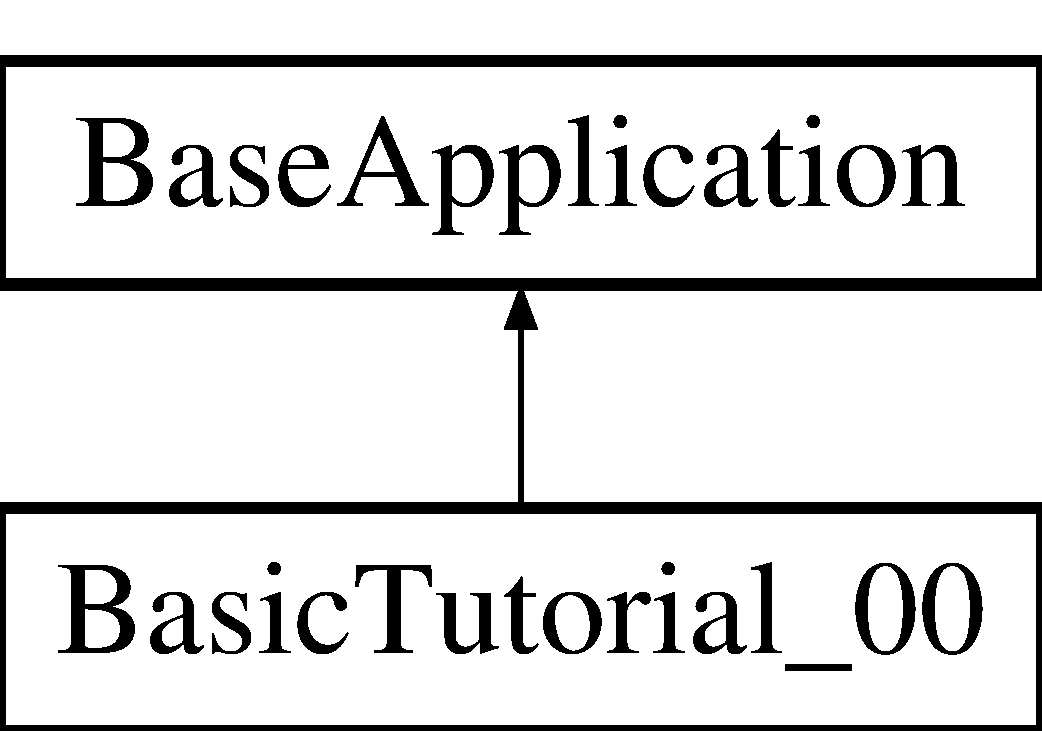
\includegraphics[height=2.382979cm]{class_base_application}
\end{center}
\end{figure}
\subsection*{Public Member Functions}
\begin{DoxyCompactItemize}
\item 
\hyperlink{class_base_application_a7c897f08816cc064568ae1ec71026719}{Base\-Application} (void)
\item 
virtual \hyperlink{class_base_application_a48e1966307d5ef8f6cbf8b6e980ad652}{$\sim$\-Base\-Application} (void)
\item 
virtual void \hyperlink{class_base_application_a8a14a65a29118dd75173aa68678a05e1}{go} (void)
\end{DoxyCompactItemize}
\subsection*{Protected Member Functions}
\begin{DoxyCompactItemize}
\item 
virtual bool \hyperlink{class_base_application_a5853d0e148cb85b0297a6885e1d33a89}{setup} ()
\item 
virtual bool \hyperlink{class_base_application_a62ed46f90e9f82cc810997647a2c587e}{configure} (void)
\item 
virtual void \hyperlink{class_base_application_ad5bc9655041e1849a4c13f444a3712bd}{choose\-Scene\-Manager} (void)
\item 
virtual void \hyperlink{class_base_application_afa9d51527763cf9aee9cd4e1b1039d55}{create\-Camera} (void)
\item 
virtual void \hyperlink{class_base_application_aff6fd9ff1ff0978cc68f19dd65be4778}{create\-Frame\-Listener} (void)
\item 
virtual void \hyperlink{class_base_application_aa97beeb4059b17d0ec22eae33286ec2d}{create\-Scene} (void)=0
\item 
virtual void \hyperlink{class_base_application_a365146059b25391fe400f5fdb94f011e}{destroy\-Scene} (void)
\item 
virtual void \hyperlink{class_base_application_a1f8f6730cae6ec769d8730b1af48486e}{create\-Viewports} (void)
\item 
virtual void \hyperlink{class_base_application_ae27301702f1e5de64619a39b1929f1f9}{setup\-Resources} (void)
\item 
virtual void \hyperlink{class_base_application_a9b77972f0f747a61e1f8ceba2ad47641}{create\-Resource\-Listener} (void)
\item 
virtual void \hyperlink{class_base_application_aaeb764e637dd87601a81a80156659d88}{load\-Resources} (void)
\item 
virtual bool \hyperlink{class_base_application_a03912a0f38b38fede7f08a2571e8fc56}{frame\-Rendering\-Queued} (const Ogre\-::\-Frame\-Event \&evt)
\item 
virtual bool \hyperlink{class_base_application_acfa977f04e435f18018ece805c1277ec}{key\-Pressed} (const O\-I\-S\-::\-Key\-Event \&arg)
\item 
virtual bool \hyperlink{class_base_application_aba5c7c9dea7a0efc58b89310bae547e5}{key\-Released} (const O\-I\-S\-::\-Key\-Event \&arg)
\item 
virtual bool \hyperlink{class_base_application_a126e59cb246b061e51eb6ce06a2ee8f4}{mouse\-Moved} (const O\-I\-S\-::\-Mouse\-Event \&arg)
\item 
virtual bool \hyperlink{class_base_application_a9255dfc1eabefd11c474ec45a6622504}{mouse\-Pressed} (const O\-I\-S\-::\-Mouse\-Event \&arg, O\-I\-S\-::\-Mouse\-Button\-I\-D id)
\item 
virtual bool \hyperlink{class_base_application_aa102c5859c14c0690c749994a446b53d}{mouse\-Released} (const O\-I\-S\-::\-Mouse\-Event \&arg, O\-I\-S\-::\-Mouse\-Button\-I\-D id)
\item 
virtual void \hyperlink{class_base_application_afacf8a797588592ef0abbad593f10cfa}{window\-Resized} (Ogre\-::\-Render\-Window $\ast$rw)
\item 
virtual void \hyperlink{class_base_application_ae0e37ac54a31ff6e51d58c7654ad1b90}{window\-Closed} (Ogre\-::\-Render\-Window $\ast$rw)
\end{DoxyCompactItemize}
\subsection*{Protected Attributes}
\begin{DoxyCompactItemize}
\item 
Ogre\-::\-Root $\ast$ \hyperlink{class_base_application_add84ba707dc6c57e6283f214b1274110}{m\-Root}
\item 
Ogre\-::\-Camera $\ast$ \hyperlink{class_base_application_a3829c6b12afe911e97e6b4524b33a38b}{m\-Camera}
\item 
Ogre\-::\-Scene\-Manager $\ast$ \hyperlink{class_base_application_a8a7684f4f9a57ed3089048ad1a913b2d}{m\-Scene\-Mgr}
\item 
Ogre\-::\-Render\-Window $\ast$ \hyperlink{class_base_application_ac5d8e9c81e036897bc82f81eff8c570f}{m\-Window}
\item 
Ogre\-::\-String \hyperlink{class_base_application_a765e0df01c141a16df3178ab4f17afe6}{m\-Resources\-Cfg}
\item 
Ogre\-::\-String \hyperlink{class_base_application_a04f2fe47fa164fd78d986dc0df70b7fb}{m\-Plugins\-Cfg}
\item 
Ogre\-Bites\-::\-Sdk\-Tray\-Manager $\ast$ \hyperlink{class_base_application_a7faa397f4f4861ee8c361a01e90b4416}{m\-Tray\-Mgr}
\item 
Ogre\-Bites\-::\-Sdk\-Camera\-Man $\ast$ \hyperlink{class_base_application_a9ae38dea6316058549151fff66a91fcd}{m\-Camera\-Man}
\item 
Ogre\-Bites\-::\-Params\-Panel $\ast$ \hyperlink{class_base_application_a6a11054ca61efdf558e0ff1b2de43a12}{m\-Details\-Panel}
\item 
bool \hyperlink{class_base_application_ac7e861799862cb645f1d78b170aef80d}{m\-Cursor\-Was\-Visible}
\item 
bool \hyperlink{class_base_application_a755f26d3a9915aaf830750d877e39d86}{m\-Shut\-Down}
\item 
O\-I\-S\-::\-Input\-Manager $\ast$ \hyperlink{class_base_application_abc9503c8462e225b5d0d55c952d9e4a9}{m\-Input\-Manager}
\item 
O\-I\-S\-::\-Mouse $\ast$ \hyperlink{class_base_application_add9b97fbe64da2814d3af113bac58c43}{m\-Mouse}
\item 
O\-I\-S\-::\-Keyboard $\ast$ \hyperlink{class_base_application_a9d6e19cf50c47379fbaae55bff28079c}{m\-Keyboard}
\end{DoxyCompactItemize}


\subsection{Constructor \& Destructor Documentation}
\hypertarget{class_base_application_a7c897f08816cc064568ae1ec71026719}{\index{Base\-Application@{Base\-Application}!Base\-Application@{Base\-Application}}
\index{Base\-Application@{Base\-Application}!BaseApplication@{Base\-Application}}
\subsubsection[{Base\-Application}]{\setlength{\rightskip}{0pt plus 5cm}Base\-Application\-::\-Base\-Application (
\begin{DoxyParamCaption}
\item[{void}]{}
\end{DoxyParamCaption}
)}}\label{class_base_application_a7c897f08816cc064568ae1ec71026719}
\hypertarget{class_base_application_a48e1966307d5ef8f6cbf8b6e980ad652}{\index{Base\-Application@{Base\-Application}!$\sim$\-Base\-Application@{$\sim$\-Base\-Application}}
\index{$\sim$\-Base\-Application@{$\sim$\-Base\-Application}!BaseApplication@{Base\-Application}}
\subsubsection[{$\sim$\-Base\-Application}]{\setlength{\rightskip}{0pt plus 5cm}Base\-Application\-::$\sim$\-Base\-Application (
\begin{DoxyParamCaption}
\item[{void}]{}
\end{DoxyParamCaption}
)\hspace{0.3cm}{\ttfamily [virtual]}}}\label{class_base_application_a48e1966307d5ef8f6cbf8b6e980ad652}


\subsection{Member Function Documentation}
\hypertarget{class_base_application_ad5bc9655041e1849a4c13f444a3712bd}{\index{Base\-Application@{Base\-Application}!choose\-Scene\-Manager@{choose\-Scene\-Manager}}
\index{choose\-Scene\-Manager@{choose\-Scene\-Manager}!BaseApplication@{Base\-Application}}
\subsubsection[{choose\-Scene\-Manager}]{\setlength{\rightskip}{0pt plus 5cm}void Base\-Application\-::choose\-Scene\-Manager (
\begin{DoxyParamCaption}
\item[{void}]{}
\end{DoxyParamCaption}
)\hspace{0.3cm}{\ttfamily [protected]}, {\ttfamily [virtual]}}}\label{class_base_application_ad5bc9655041e1849a4c13f444a3712bd}


Reimplemented in \hyperlink{class_basic_tutorial__00_aba97a29d983586d2dc8e108d3bccf721}{Basic\-Tutorial\-\_\-00}.

\hypertarget{class_base_application_a62ed46f90e9f82cc810997647a2c587e}{\index{Base\-Application@{Base\-Application}!configure@{configure}}
\index{configure@{configure}!BaseApplication@{Base\-Application}}
\subsubsection[{configure}]{\setlength{\rightskip}{0pt plus 5cm}bool Base\-Application\-::configure (
\begin{DoxyParamCaption}
\item[{void}]{}
\end{DoxyParamCaption}
)\hspace{0.3cm}{\ttfamily [protected]}, {\ttfamily [virtual]}}}\label{class_base_application_a62ed46f90e9f82cc810997647a2c587e}
\hypertarget{class_base_application_afa9d51527763cf9aee9cd4e1b1039d55}{\index{Base\-Application@{Base\-Application}!create\-Camera@{create\-Camera}}
\index{create\-Camera@{create\-Camera}!BaseApplication@{Base\-Application}}
\subsubsection[{create\-Camera}]{\setlength{\rightskip}{0pt plus 5cm}void Base\-Application\-::create\-Camera (
\begin{DoxyParamCaption}
\item[{void}]{}
\end{DoxyParamCaption}
)\hspace{0.3cm}{\ttfamily [protected]}, {\ttfamily [virtual]}}}\label{class_base_application_afa9d51527763cf9aee9cd4e1b1039d55}


Reimplemented in \hyperlink{class_basic_tutorial__00_a1bf709417d654dffc2ea10987412b912}{Basic\-Tutorial\-\_\-00}.

\hypertarget{class_base_application_aff6fd9ff1ff0978cc68f19dd65be4778}{\index{Base\-Application@{Base\-Application}!create\-Frame\-Listener@{create\-Frame\-Listener}}
\index{create\-Frame\-Listener@{create\-Frame\-Listener}!BaseApplication@{Base\-Application}}
\subsubsection[{create\-Frame\-Listener}]{\setlength{\rightskip}{0pt plus 5cm}void Base\-Application\-::create\-Frame\-Listener (
\begin{DoxyParamCaption}
\item[{void}]{}
\end{DoxyParamCaption}
)\hspace{0.3cm}{\ttfamily [protected]}, {\ttfamily [virtual]}}}\label{class_base_application_aff6fd9ff1ff0978cc68f19dd65be4778}
\hypertarget{class_base_application_a9b77972f0f747a61e1f8ceba2ad47641}{\index{Base\-Application@{Base\-Application}!create\-Resource\-Listener@{create\-Resource\-Listener}}
\index{create\-Resource\-Listener@{create\-Resource\-Listener}!BaseApplication@{Base\-Application}}
\subsubsection[{create\-Resource\-Listener}]{\setlength{\rightskip}{0pt plus 5cm}void Base\-Application\-::create\-Resource\-Listener (
\begin{DoxyParamCaption}
\item[{void}]{}
\end{DoxyParamCaption}
)\hspace{0.3cm}{\ttfamily [protected]}, {\ttfamily [virtual]}}}\label{class_base_application_a9b77972f0f747a61e1f8ceba2ad47641}
\hypertarget{class_base_application_aa97beeb4059b17d0ec22eae33286ec2d}{\index{Base\-Application@{Base\-Application}!create\-Scene@{create\-Scene}}
\index{create\-Scene@{create\-Scene}!BaseApplication@{Base\-Application}}
\subsubsection[{create\-Scene}]{\setlength{\rightskip}{0pt plus 5cm}virtual void Base\-Application\-::create\-Scene (
\begin{DoxyParamCaption}
\item[{void}]{}
\end{DoxyParamCaption}
)\hspace{0.3cm}{\ttfamily [protected]}, {\ttfamily [pure virtual]}}}\label{class_base_application_aa97beeb4059b17d0ec22eae33286ec2d}


Implemented in \hyperlink{class_basic_tutorial__00_a15a3d4673724ec99077ce992f996a550}{Basic\-Tutorial\-\_\-00}.

\hypertarget{class_base_application_a1f8f6730cae6ec769d8730b1af48486e}{\index{Base\-Application@{Base\-Application}!create\-Viewports@{create\-Viewports}}
\index{create\-Viewports@{create\-Viewports}!BaseApplication@{Base\-Application}}
\subsubsection[{create\-Viewports}]{\setlength{\rightskip}{0pt plus 5cm}void Base\-Application\-::create\-Viewports (
\begin{DoxyParamCaption}
\item[{void}]{}
\end{DoxyParamCaption}
)\hspace{0.3cm}{\ttfamily [protected]}, {\ttfamily [virtual]}}}\label{class_base_application_a1f8f6730cae6ec769d8730b1af48486e}


Reimplemented in \hyperlink{class_basic_tutorial__00_adc2454d9f8226e0958ecf702f355846e}{Basic\-Tutorial\-\_\-00}.

\hypertarget{class_base_application_a365146059b25391fe400f5fdb94f011e}{\index{Base\-Application@{Base\-Application}!destroy\-Scene@{destroy\-Scene}}
\index{destroy\-Scene@{destroy\-Scene}!BaseApplication@{Base\-Application}}
\subsubsection[{destroy\-Scene}]{\setlength{\rightskip}{0pt plus 5cm}void Base\-Application\-::destroy\-Scene (
\begin{DoxyParamCaption}
\item[{void}]{}
\end{DoxyParamCaption}
)\hspace{0.3cm}{\ttfamily [protected]}, {\ttfamily [virtual]}}}\label{class_base_application_a365146059b25391fe400f5fdb94f011e}
\hypertarget{class_base_application_a03912a0f38b38fede7f08a2571e8fc56}{\index{Base\-Application@{Base\-Application}!frame\-Rendering\-Queued@{frame\-Rendering\-Queued}}
\index{frame\-Rendering\-Queued@{frame\-Rendering\-Queued}!BaseApplication@{Base\-Application}}
\subsubsection[{frame\-Rendering\-Queued}]{\setlength{\rightskip}{0pt plus 5cm}bool Base\-Application\-::frame\-Rendering\-Queued (
\begin{DoxyParamCaption}
\item[{const Ogre\-::\-Frame\-Event \&}]{evt}
\end{DoxyParamCaption}
)\hspace{0.3cm}{\ttfamily [protected]}, {\ttfamily [virtual]}}}\label{class_base_application_a03912a0f38b38fede7f08a2571e8fc56}
\hypertarget{class_base_application_a8a14a65a29118dd75173aa68678a05e1}{\index{Base\-Application@{Base\-Application}!go@{go}}
\index{go@{go}!BaseApplication@{Base\-Application}}
\subsubsection[{go}]{\setlength{\rightskip}{0pt plus 5cm}void Base\-Application\-::go (
\begin{DoxyParamCaption}
\item[{void}]{}
\end{DoxyParamCaption}
)\hspace{0.3cm}{\ttfamily [virtual]}}}\label{class_base_application_a8a14a65a29118dd75173aa68678a05e1}
\hypertarget{class_base_application_acfa977f04e435f18018ece805c1277ec}{\index{Base\-Application@{Base\-Application}!key\-Pressed@{key\-Pressed}}
\index{key\-Pressed@{key\-Pressed}!BaseApplication@{Base\-Application}}
\subsubsection[{key\-Pressed}]{\setlength{\rightskip}{0pt plus 5cm}bool Base\-Application\-::key\-Pressed (
\begin{DoxyParamCaption}
\item[{const O\-I\-S\-::\-Key\-Event \&}]{arg}
\end{DoxyParamCaption}
)\hspace{0.3cm}{\ttfamily [protected]}, {\ttfamily [virtual]}}}\label{class_base_application_acfa977f04e435f18018ece805c1277ec}
\hypertarget{class_base_application_aba5c7c9dea7a0efc58b89310bae547e5}{\index{Base\-Application@{Base\-Application}!key\-Released@{key\-Released}}
\index{key\-Released@{key\-Released}!BaseApplication@{Base\-Application}}
\subsubsection[{key\-Released}]{\setlength{\rightskip}{0pt plus 5cm}bool Base\-Application\-::key\-Released (
\begin{DoxyParamCaption}
\item[{const O\-I\-S\-::\-Key\-Event \&}]{arg}
\end{DoxyParamCaption}
)\hspace{0.3cm}{\ttfamily [protected]}, {\ttfamily [virtual]}}}\label{class_base_application_aba5c7c9dea7a0efc58b89310bae547e5}
\hypertarget{class_base_application_aaeb764e637dd87601a81a80156659d88}{\index{Base\-Application@{Base\-Application}!load\-Resources@{load\-Resources}}
\index{load\-Resources@{load\-Resources}!BaseApplication@{Base\-Application}}
\subsubsection[{load\-Resources}]{\setlength{\rightskip}{0pt plus 5cm}void Base\-Application\-::load\-Resources (
\begin{DoxyParamCaption}
\item[{void}]{}
\end{DoxyParamCaption}
)\hspace{0.3cm}{\ttfamily [protected]}, {\ttfamily [virtual]}}}\label{class_base_application_aaeb764e637dd87601a81a80156659d88}
\hypertarget{class_base_application_a126e59cb246b061e51eb6ce06a2ee8f4}{\index{Base\-Application@{Base\-Application}!mouse\-Moved@{mouse\-Moved}}
\index{mouse\-Moved@{mouse\-Moved}!BaseApplication@{Base\-Application}}
\subsubsection[{mouse\-Moved}]{\setlength{\rightskip}{0pt plus 5cm}bool Base\-Application\-::mouse\-Moved (
\begin{DoxyParamCaption}
\item[{const O\-I\-S\-::\-Mouse\-Event \&}]{arg}
\end{DoxyParamCaption}
)\hspace{0.3cm}{\ttfamily [protected]}, {\ttfamily [virtual]}}}\label{class_base_application_a126e59cb246b061e51eb6ce06a2ee8f4}
\hypertarget{class_base_application_a9255dfc1eabefd11c474ec45a6622504}{\index{Base\-Application@{Base\-Application}!mouse\-Pressed@{mouse\-Pressed}}
\index{mouse\-Pressed@{mouse\-Pressed}!BaseApplication@{Base\-Application}}
\subsubsection[{mouse\-Pressed}]{\setlength{\rightskip}{0pt plus 5cm}bool Base\-Application\-::mouse\-Pressed (
\begin{DoxyParamCaption}
\item[{const O\-I\-S\-::\-Mouse\-Event \&}]{arg, }
\item[{O\-I\-S\-::\-Mouse\-Button\-I\-D}]{id}
\end{DoxyParamCaption}
)\hspace{0.3cm}{\ttfamily [protected]}, {\ttfamily [virtual]}}}\label{class_base_application_a9255dfc1eabefd11c474ec45a6622504}
\hypertarget{class_base_application_aa102c5859c14c0690c749994a446b53d}{\index{Base\-Application@{Base\-Application}!mouse\-Released@{mouse\-Released}}
\index{mouse\-Released@{mouse\-Released}!BaseApplication@{Base\-Application}}
\subsubsection[{mouse\-Released}]{\setlength{\rightskip}{0pt plus 5cm}bool Base\-Application\-::mouse\-Released (
\begin{DoxyParamCaption}
\item[{const O\-I\-S\-::\-Mouse\-Event \&}]{arg, }
\item[{O\-I\-S\-::\-Mouse\-Button\-I\-D}]{id}
\end{DoxyParamCaption}
)\hspace{0.3cm}{\ttfamily [protected]}, {\ttfamily [virtual]}}}\label{class_base_application_aa102c5859c14c0690c749994a446b53d}
\hypertarget{class_base_application_a5853d0e148cb85b0297a6885e1d33a89}{\index{Base\-Application@{Base\-Application}!setup@{setup}}
\index{setup@{setup}!BaseApplication@{Base\-Application}}
\subsubsection[{setup}]{\setlength{\rightskip}{0pt plus 5cm}bool Base\-Application\-::setup (
\begin{DoxyParamCaption}
\item[{void}]{}
\end{DoxyParamCaption}
)\hspace{0.3cm}{\ttfamily [protected]}, {\ttfamily [virtual]}}}\label{class_base_application_a5853d0e148cb85b0297a6885e1d33a89}
\hypertarget{class_base_application_ae27301702f1e5de64619a39b1929f1f9}{\index{Base\-Application@{Base\-Application}!setup\-Resources@{setup\-Resources}}
\index{setup\-Resources@{setup\-Resources}!BaseApplication@{Base\-Application}}
\subsubsection[{setup\-Resources}]{\setlength{\rightskip}{0pt plus 5cm}void Base\-Application\-::setup\-Resources (
\begin{DoxyParamCaption}
\item[{void}]{}
\end{DoxyParamCaption}
)\hspace{0.3cm}{\ttfamily [protected]}, {\ttfamily [virtual]}}}\label{class_base_application_ae27301702f1e5de64619a39b1929f1f9}
\hypertarget{class_base_application_ae0e37ac54a31ff6e51d58c7654ad1b90}{\index{Base\-Application@{Base\-Application}!window\-Closed@{window\-Closed}}
\index{window\-Closed@{window\-Closed}!BaseApplication@{Base\-Application}}
\subsubsection[{window\-Closed}]{\setlength{\rightskip}{0pt plus 5cm}void Base\-Application\-::window\-Closed (
\begin{DoxyParamCaption}
\item[{Ogre\-::\-Render\-Window $\ast$}]{rw}
\end{DoxyParamCaption}
)\hspace{0.3cm}{\ttfamily [protected]}, {\ttfamily [virtual]}}}\label{class_base_application_ae0e37ac54a31ff6e51d58c7654ad1b90}
\hypertarget{class_base_application_afacf8a797588592ef0abbad593f10cfa}{\index{Base\-Application@{Base\-Application}!window\-Resized@{window\-Resized}}
\index{window\-Resized@{window\-Resized}!BaseApplication@{Base\-Application}}
\subsubsection[{window\-Resized}]{\setlength{\rightskip}{0pt plus 5cm}void Base\-Application\-::window\-Resized (
\begin{DoxyParamCaption}
\item[{Ogre\-::\-Render\-Window $\ast$}]{rw}
\end{DoxyParamCaption}
)\hspace{0.3cm}{\ttfamily [protected]}, {\ttfamily [virtual]}}}\label{class_base_application_afacf8a797588592ef0abbad593f10cfa}


\subsection{Member Data Documentation}
\hypertarget{class_base_application_a3829c6b12afe911e97e6b4524b33a38b}{\index{Base\-Application@{Base\-Application}!m\-Camera@{m\-Camera}}
\index{m\-Camera@{m\-Camera}!BaseApplication@{Base\-Application}}
\subsubsection[{m\-Camera}]{\setlength{\rightskip}{0pt plus 5cm}Ogre\-::\-Camera$\ast$ Base\-Application\-::m\-Camera\hspace{0.3cm}{\ttfamily [protected]}}}\label{class_base_application_a3829c6b12afe911e97e6b4524b33a38b}
\hypertarget{class_base_application_a9ae38dea6316058549151fff66a91fcd}{\index{Base\-Application@{Base\-Application}!m\-Camera\-Man@{m\-Camera\-Man}}
\index{m\-Camera\-Man@{m\-Camera\-Man}!BaseApplication@{Base\-Application}}
\subsubsection[{m\-Camera\-Man}]{\setlength{\rightskip}{0pt plus 5cm}Ogre\-Bites\-::\-Sdk\-Camera\-Man$\ast$ Base\-Application\-::m\-Camera\-Man\hspace{0.3cm}{\ttfamily [protected]}}}\label{class_base_application_a9ae38dea6316058549151fff66a91fcd}
\hypertarget{class_base_application_ac7e861799862cb645f1d78b170aef80d}{\index{Base\-Application@{Base\-Application}!m\-Cursor\-Was\-Visible@{m\-Cursor\-Was\-Visible}}
\index{m\-Cursor\-Was\-Visible@{m\-Cursor\-Was\-Visible}!BaseApplication@{Base\-Application}}
\subsubsection[{m\-Cursor\-Was\-Visible}]{\setlength{\rightskip}{0pt plus 5cm}bool Base\-Application\-::m\-Cursor\-Was\-Visible\hspace{0.3cm}{\ttfamily [protected]}}}\label{class_base_application_ac7e861799862cb645f1d78b170aef80d}
\hypertarget{class_base_application_a6a11054ca61efdf558e0ff1b2de43a12}{\index{Base\-Application@{Base\-Application}!m\-Details\-Panel@{m\-Details\-Panel}}
\index{m\-Details\-Panel@{m\-Details\-Panel}!BaseApplication@{Base\-Application}}
\subsubsection[{m\-Details\-Panel}]{\setlength{\rightskip}{0pt plus 5cm}Ogre\-Bites\-::\-Params\-Panel$\ast$ Base\-Application\-::m\-Details\-Panel\hspace{0.3cm}{\ttfamily [protected]}}}\label{class_base_application_a6a11054ca61efdf558e0ff1b2de43a12}
\hypertarget{class_base_application_abc9503c8462e225b5d0d55c952d9e4a9}{\index{Base\-Application@{Base\-Application}!m\-Input\-Manager@{m\-Input\-Manager}}
\index{m\-Input\-Manager@{m\-Input\-Manager}!BaseApplication@{Base\-Application}}
\subsubsection[{m\-Input\-Manager}]{\setlength{\rightskip}{0pt plus 5cm}O\-I\-S\-::\-Input\-Manager$\ast$ Base\-Application\-::m\-Input\-Manager\hspace{0.3cm}{\ttfamily [protected]}}}\label{class_base_application_abc9503c8462e225b5d0d55c952d9e4a9}
\hypertarget{class_base_application_a9d6e19cf50c47379fbaae55bff28079c}{\index{Base\-Application@{Base\-Application}!m\-Keyboard@{m\-Keyboard}}
\index{m\-Keyboard@{m\-Keyboard}!BaseApplication@{Base\-Application}}
\subsubsection[{m\-Keyboard}]{\setlength{\rightskip}{0pt plus 5cm}O\-I\-S\-::\-Keyboard$\ast$ Base\-Application\-::m\-Keyboard\hspace{0.3cm}{\ttfamily [protected]}}}\label{class_base_application_a9d6e19cf50c47379fbaae55bff28079c}
\hypertarget{class_base_application_add9b97fbe64da2814d3af113bac58c43}{\index{Base\-Application@{Base\-Application}!m\-Mouse@{m\-Mouse}}
\index{m\-Mouse@{m\-Mouse}!BaseApplication@{Base\-Application}}
\subsubsection[{m\-Mouse}]{\setlength{\rightskip}{0pt plus 5cm}O\-I\-S\-::\-Mouse$\ast$ Base\-Application\-::m\-Mouse\hspace{0.3cm}{\ttfamily [protected]}}}\label{class_base_application_add9b97fbe64da2814d3af113bac58c43}
\hypertarget{class_base_application_a04f2fe47fa164fd78d986dc0df70b7fb}{\index{Base\-Application@{Base\-Application}!m\-Plugins\-Cfg@{m\-Plugins\-Cfg}}
\index{m\-Plugins\-Cfg@{m\-Plugins\-Cfg}!BaseApplication@{Base\-Application}}
\subsubsection[{m\-Plugins\-Cfg}]{\setlength{\rightskip}{0pt plus 5cm}Ogre\-::\-String Base\-Application\-::m\-Plugins\-Cfg\hspace{0.3cm}{\ttfamily [protected]}}}\label{class_base_application_a04f2fe47fa164fd78d986dc0df70b7fb}
\hypertarget{class_base_application_a765e0df01c141a16df3178ab4f17afe6}{\index{Base\-Application@{Base\-Application}!m\-Resources\-Cfg@{m\-Resources\-Cfg}}
\index{m\-Resources\-Cfg@{m\-Resources\-Cfg}!BaseApplication@{Base\-Application}}
\subsubsection[{m\-Resources\-Cfg}]{\setlength{\rightskip}{0pt plus 5cm}Ogre\-::\-String Base\-Application\-::m\-Resources\-Cfg\hspace{0.3cm}{\ttfamily [protected]}}}\label{class_base_application_a765e0df01c141a16df3178ab4f17afe6}
\hypertarget{class_base_application_add84ba707dc6c57e6283f214b1274110}{\index{Base\-Application@{Base\-Application}!m\-Root@{m\-Root}}
\index{m\-Root@{m\-Root}!BaseApplication@{Base\-Application}}
\subsubsection[{m\-Root}]{\setlength{\rightskip}{0pt plus 5cm}Ogre\-::\-Root$\ast$ Base\-Application\-::m\-Root\hspace{0.3cm}{\ttfamily [protected]}}}\label{class_base_application_add84ba707dc6c57e6283f214b1274110}
\hypertarget{class_base_application_a8a7684f4f9a57ed3089048ad1a913b2d}{\index{Base\-Application@{Base\-Application}!m\-Scene\-Mgr@{m\-Scene\-Mgr}}
\index{m\-Scene\-Mgr@{m\-Scene\-Mgr}!BaseApplication@{Base\-Application}}
\subsubsection[{m\-Scene\-Mgr}]{\setlength{\rightskip}{0pt plus 5cm}Ogre\-::\-Scene\-Manager$\ast$ Base\-Application\-::m\-Scene\-Mgr\hspace{0.3cm}{\ttfamily [protected]}}}\label{class_base_application_a8a7684f4f9a57ed3089048ad1a913b2d}
\hypertarget{class_base_application_a755f26d3a9915aaf830750d877e39d86}{\index{Base\-Application@{Base\-Application}!m\-Shut\-Down@{m\-Shut\-Down}}
\index{m\-Shut\-Down@{m\-Shut\-Down}!BaseApplication@{Base\-Application}}
\subsubsection[{m\-Shut\-Down}]{\setlength{\rightskip}{0pt plus 5cm}bool Base\-Application\-::m\-Shut\-Down\hspace{0.3cm}{\ttfamily [protected]}}}\label{class_base_application_a755f26d3a9915aaf830750d877e39d86}
\hypertarget{class_base_application_a7faa397f4f4861ee8c361a01e90b4416}{\index{Base\-Application@{Base\-Application}!m\-Tray\-Mgr@{m\-Tray\-Mgr}}
\index{m\-Tray\-Mgr@{m\-Tray\-Mgr}!BaseApplication@{Base\-Application}}
\subsubsection[{m\-Tray\-Mgr}]{\setlength{\rightskip}{0pt plus 5cm}Ogre\-Bites\-::\-Sdk\-Tray\-Manager$\ast$ Base\-Application\-::m\-Tray\-Mgr\hspace{0.3cm}{\ttfamily [protected]}}}\label{class_base_application_a7faa397f4f4861ee8c361a01e90b4416}
\hypertarget{class_base_application_ac5d8e9c81e036897bc82f81eff8c570f}{\index{Base\-Application@{Base\-Application}!m\-Window@{m\-Window}}
\index{m\-Window@{m\-Window}!BaseApplication@{Base\-Application}}
\subsubsection[{m\-Window}]{\setlength{\rightskip}{0pt plus 5cm}Ogre\-::\-Render\-Window$\ast$ Base\-Application\-::m\-Window\hspace{0.3cm}{\ttfamily [protected]}}}\label{class_base_application_ac5d8e9c81e036897bc82f81eff8c570f}


The documentation for this class was generated from the following files\-:\begin{DoxyCompactItemize}
\item 
source/\hyperlink{_base_application_8h}{Base\-Application.\-h}\item 
source/\hyperlink{_base_application_8cpp}{Base\-Application.\-cpp}\end{DoxyCompactItemize}

\hypertarget{class_basic_tutorial__00}{\section{Basic\-Tutorial\-\_\-00 Class Reference}
\label{class_basic_tutorial__00}\index{Basic\-Tutorial\-\_\-00@{Basic\-Tutorial\-\_\-00}}
}


3\-D Game Programming \par
 My Name\-: Wei-\/\-Sheng Zeng \par
 My I\-D\-: 9917144 \par
 My Email\-: \href{mailto:cvs5689@gmail.com}{\tt cvs5689@gmail.\-com}  




{\ttfamily \#include $<$Tutorial\-Application.\-h$>$}

Inheritance diagram for Basic\-Tutorial\-\_\-00\-:\begin{figure}[H]
\begin{center}
\leavevmode
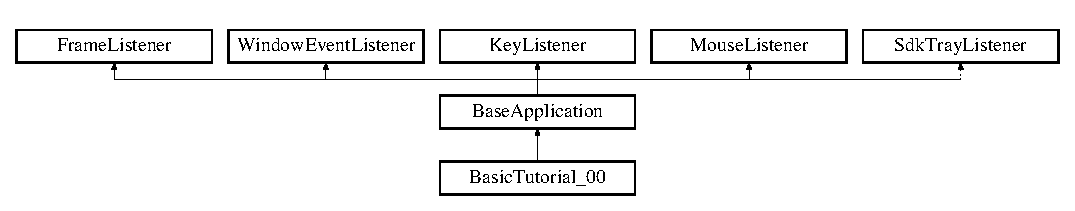
\includegraphics[height=2.382979cm]{class_basic_tutorial__00}
\end{center}
\end{figure}
\subsection*{Public Member Functions}
\begin{DoxyCompactItemize}
\item 
\hyperlink{class_basic_tutorial__00_a6b55068822076b28e7819b1878e95684}{Basic\-Tutorial\-\_\-00} (void)
\item 
virtual void \hyperlink{class_basic_tutorial__00_adc2454d9f8226e0958ecf702f355846e}{create\-Viewports} (void)
\item 
virtual void \hyperlink{class_basic_tutorial__00_a15a3d4673724ec99077ce992f996a550}{create\-Scene} (void)
\item 
virtual void \hyperlink{class_basic_tutorial__00_a1bf709417d654dffc2ea10987412b912}{create\-Camera} (void)
\item 
virtual void \hyperlink{class_basic_tutorial__00_aba97a29d983586d2dc8e108d3bccf721}{choose\-Scene\-Manager} (void)
\end{DoxyCompactItemize}
\subsection*{Additional Inherited Members}


\subsection{Detailed Description}
3\-D Game Programming \par
 My Name\-: Wei-\/\-Sheng Zeng \par
 My I\-D\-: 9917144 \par
 My Email\-: \href{mailto:cvs5689@gmail.com}{\tt cvs5689@gmail.\-com} 

This is an assignment of 3\-D Game Programming 

\subsection{Constructor \& Destructor Documentation}
\hypertarget{class_basic_tutorial__00_a6b55068822076b28e7819b1878e95684}{\index{Basic\-Tutorial\-\_\-00@{Basic\-Tutorial\-\_\-00}!Basic\-Tutorial\-\_\-00@{Basic\-Tutorial\-\_\-00}}
\index{Basic\-Tutorial\-\_\-00@{Basic\-Tutorial\-\_\-00}!BasicTutorial_00@{Basic\-Tutorial\-\_\-00}}
\subsubsection[{Basic\-Tutorial\-\_\-00}]{\setlength{\rightskip}{0pt plus 5cm}Basic\-Tutorial\-\_\-00\-::\-Basic\-Tutorial\-\_\-00 (
\begin{DoxyParamCaption}
\item[{void}]{}
\end{DoxyParamCaption}
)}}\label{class_basic_tutorial__00_a6b55068822076b28e7819b1878e95684}


\subsection{Member Function Documentation}
\hypertarget{class_basic_tutorial__00_aba97a29d983586d2dc8e108d3bccf721}{\index{Basic\-Tutorial\-\_\-00@{Basic\-Tutorial\-\_\-00}!choose\-Scene\-Manager@{choose\-Scene\-Manager}}
\index{choose\-Scene\-Manager@{choose\-Scene\-Manager}!BasicTutorial_00@{Basic\-Tutorial\-\_\-00}}
\subsubsection[{choose\-Scene\-Manager}]{\setlength{\rightskip}{0pt plus 5cm}void Basic\-Tutorial\-\_\-00\-::choose\-Scene\-Manager (
\begin{DoxyParamCaption}
\item[{void}]{}
\end{DoxyParamCaption}
)\hspace{0.3cm}{\ttfamily [virtual]}}}\label{class_basic_tutorial__00_aba97a29d983586d2dc8e108d3bccf721}
Simply create two scene manager. 

Reimplemented from \hyperlink{class_base_application_ad5bc9655041e1849a4c13f444a3712bd}{Base\-Application}.

\hypertarget{class_basic_tutorial__00_a1bf709417d654dffc2ea10987412b912}{\index{Basic\-Tutorial\-\_\-00@{Basic\-Tutorial\-\_\-00}!create\-Camera@{create\-Camera}}
\index{create\-Camera@{create\-Camera}!BasicTutorial_00@{Basic\-Tutorial\-\_\-00}}
\subsubsection[{create\-Camera}]{\setlength{\rightskip}{0pt plus 5cm}void Basic\-Tutorial\-\_\-00\-::create\-Camera (
\begin{DoxyParamCaption}
\item[{void}]{}
\end{DoxyParamCaption}
)\hspace{0.3cm}{\ttfamily [virtual]}}}\label{class_basic_tutorial__00_a1bf709417d654dffc2ea10987412b912}
Call create\-Camera\-\_\-00 and create\-Camera\-\_\-01 to setup two cameras and set camera\-\_\-00 to be main. 

Reimplemented from \hyperlink{class_base_application_afa9d51527763cf9aee9cd4e1b1039d55}{Base\-Application}.

\hypertarget{class_basic_tutorial__00_a15a3d4673724ec99077ce992f996a550}{\index{Basic\-Tutorial\-\_\-00@{Basic\-Tutorial\-\_\-00}!create\-Scene@{create\-Scene}}
\index{create\-Scene@{create\-Scene}!BasicTutorial_00@{Basic\-Tutorial\-\_\-00}}
\subsubsection[{create\-Scene}]{\setlength{\rightskip}{0pt plus 5cm}void Basic\-Tutorial\-\_\-00\-::create\-Scene (
\begin{DoxyParamCaption}
\item[{void}]{}
\end{DoxyParamCaption}
)\hspace{0.3cm}{\ttfamily [virtual]}}}\label{class_basic_tutorial__00_a15a3d4673724ec99077ce992f996a550}
Call create\-Scene\-\_\-00 and create\-Scene\-\_\-01 to create two scenes. 

Implements \hyperlink{class_base_application_aa97beeb4059b17d0ec22eae33286ec2d}{Base\-Application}.

\hypertarget{class_basic_tutorial__00_adc2454d9f8226e0958ecf702f355846e}{\index{Basic\-Tutorial\-\_\-00@{Basic\-Tutorial\-\_\-00}!create\-Viewports@{create\-Viewports}}
\index{create\-Viewports@{create\-Viewports}!BasicTutorial_00@{Basic\-Tutorial\-\_\-00}}
\subsubsection[{create\-Viewports}]{\setlength{\rightskip}{0pt plus 5cm}void Basic\-Tutorial\-\_\-00\-::create\-Viewports (
\begin{DoxyParamCaption}
\item[{void}]{}
\end{DoxyParamCaption}
)\hspace{0.3cm}{\ttfamily [virtual]}}}\label{class_basic_tutorial__00_adc2454d9f8226e0958ecf702f355846e}
Set up two viewport with create\-Viewport\-\_\-00 and create\-Viewport\-\_\-01. 

Reimplemented from \hyperlink{class_base_application_a1f8f6730cae6ec769d8730b1af48486e}{Base\-Application}.



The documentation for this class was generated from the following files\-:\begin{DoxyCompactItemize}
\item 
source/\hyperlink{_tutorial_application_8h}{Tutorial\-Application.\-h}\item 
source/\hyperlink{_tutorial_application_8cpp}{Tutorial\-Application.\-cpp}\end{DoxyCompactItemize}

\chapter{File Documentation}
\hypertarget{_base_application_8cpp}{\section{source/\-Base\-Application.cpp File Reference}
\label{_base_application_8cpp}\index{source/\-Base\-Application.\-cpp@{source/\-Base\-Application.\-cpp}}
}
{\ttfamily \#include \char`\"{}Base\-Application.\-h\char`\"{}}\\*

\hypertarget{_base_application_8h}{\section{source/\-Base\-Application.h File Reference}
\label{_base_application_8h}\index{source/\-Base\-Application.\-h@{source/\-Base\-Application.\-h}}
}
{\ttfamily \#include $<$Ogre\-Camera.\-h$>$}\\*
{\ttfamily \#include $<$Ogre\-Entity.\-h$>$}\\*
{\ttfamily \#include $<$Ogre\-Log\-Manager.\-h$>$}\\*
{\ttfamily \#include $<$Ogre\-Root.\-h$>$}\\*
{\ttfamily \#include $<$Ogre\-Viewport.\-h$>$}\\*
{\ttfamily \#include $<$Ogre\-Scene\-Manager.\-h$>$}\\*
{\ttfamily \#include $<$Ogre\-Render\-Window.\-h$>$}\\*
{\ttfamily \#include $<$Ogre\-Config\-File.\-h$>$}\\*
{\ttfamily \#include $<$O\-I\-S\-Events.\-h$>$}\\*
{\ttfamily \#include $<$O\-I\-S\-Input\-Manager.\-h$>$}\\*
{\ttfamily \#include $<$O\-I\-S\-Keyboard.\-h$>$}\\*
{\ttfamily \#include $<$O\-I\-S\-Mouse.\-h$>$}\\*
{\ttfamily \#include $<$Sdk\-Trays.\-h$>$}\\*
{\ttfamily \#include $<$Sdk\-Camera\-Man.\-h$>$}\\*
\subsection*{Classes}
\begin{DoxyCompactItemize}
\item 
class \hyperlink{class_base_application}{Base\-Application}
\end{DoxyCompactItemize}

\hypertarget{_basic_tools_8cpp}{\section{source/\-Basic\-Tools.cpp File Reference}
\label{_basic_tools_8cpp}\index{source/\-Basic\-Tools.\-cpp@{source/\-Basic\-Tools.\-cpp}}
}
{\ttfamily \#include \char`\"{}Basic\-Tools.\-h\char`\"{}}\\*
\subsection*{Functions}
\begin{DoxyCompactItemize}
\item 
void \hyperlink{_basic_tools_8cpp_ad63cd10373a31b26af05b94261684122}{gen\-Name\-Using\-Index} (const Ogre\-::\-String \&prefix, int index, Ogre\-::\-String \&out\-\_\-name)
\end{DoxyCompactItemize}


\subsection{Function Documentation}
\hypertarget{_basic_tools_8cpp_ad63cd10373a31b26af05b94261684122}{\index{Basic\-Tools.\-cpp@{Basic\-Tools.\-cpp}!gen\-Name\-Using\-Index@{gen\-Name\-Using\-Index}}
\index{gen\-Name\-Using\-Index@{gen\-Name\-Using\-Index}!BasicTools.cpp@{Basic\-Tools.\-cpp}}
\subsubsection[{gen\-Name\-Using\-Index}]{\setlength{\rightskip}{0pt plus 5cm}void gen\-Name\-Using\-Index (
\begin{DoxyParamCaption}
\item[{const Ogre\-::\-String \&}]{prefix, }
\item[{int}]{index, }
\item[{Ogre\-::\-String \&}]{out\-\_\-name}
\end{DoxyParamCaption}
)}}\label{_basic_tools_8cpp_ad63cd10373a31b26af05b94261684122}

\hypertarget{_basic_tools_8h}{\section{source/\-Basic\-Tools.h File Reference}
\label{_basic_tools_8h}\index{source/\-Basic\-Tools.\-h@{source/\-Basic\-Tools.\-h}}
}
{\ttfamily \#include $<$Ogre\-Camera.\-h$>$}\\*
{\ttfamily \#include $<$Ogre\-Entity.\-h$>$}\\*
{\ttfamily \#include $<$Ogre\-Log\-Manager.\-h$>$}\\*
{\ttfamily \#include $<$Ogre\-Root.\-h$>$}\\*
{\ttfamily \#include $<$Ogre\-Viewport.\-h$>$}\\*
{\ttfamily \#include $<$Ogre\-Scene\-Manager.\-h$>$}\\*
{\ttfamily \#include $<$Ogre\-Render\-Window.\-h$>$}\\*
{\ttfamily \#include $<$Ogre\-Config\-File.\-h$>$}\\*
\subsection*{Functions}
\begin{DoxyCompactItemize}
\item 
void \hyperlink{_basic_tools_8h_ad63cd10373a31b26af05b94261684122}{gen\-Name\-Using\-Index} (const Ogre\-::\-String \&prefix, int index, Ogre\-::\-String \&out\-\_\-name)
\end{DoxyCompactItemize}


\subsection{Function Documentation}
\hypertarget{_basic_tools_8h_ad63cd10373a31b26af05b94261684122}{\index{Basic\-Tools.\-h@{Basic\-Tools.\-h}!gen\-Name\-Using\-Index@{gen\-Name\-Using\-Index}}
\index{gen\-Name\-Using\-Index@{gen\-Name\-Using\-Index}!BasicTools.h@{Basic\-Tools.\-h}}
\subsubsection[{gen\-Name\-Using\-Index}]{\setlength{\rightskip}{0pt plus 5cm}void gen\-Name\-Using\-Index (
\begin{DoxyParamCaption}
\item[{const Ogre\-::\-String \&}]{prefix, }
\item[{int}]{index, }
\item[{Ogre\-::\-String \&}]{out\-\_\-name}
\end{DoxyParamCaption}
)}}\label{_basic_tools_8h_ad63cd10373a31b26af05b94261684122}

\hypertarget{_tutorial_application_8cpp}{\section{source/\-Tutorial\-Application.cpp File Reference}
\label{_tutorial_application_8cpp}\index{source/\-Tutorial\-Application.\-cpp@{source/\-Tutorial\-Application.\-cpp}}
}
{\ttfamily \#include \char`\"{}Tutorial\-Application.\-h\char`\"{}}\\*
{\ttfamily \#include \char`\"{}Basic\-Tools.\-h\char`\"{}}\\*
\subsection*{Functions}
\begin{DoxyCompactItemize}
\item 
int \hyperlink{_tutorial_application_8cpp_a0ddf1224851353fc92bfbff6f499fa97}{main} (int argc, char $\ast$argv\mbox{[}$\,$\mbox{]})
\end{DoxyCompactItemize}


\subsection{Function Documentation}
\hypertarget{_tutorial_application_8cpp_a0ddf1224851353fc92bfbff6f499fa97}{\index{Tutorial\-Application.\-cpp@{Tutorial\-Application.\-cpp}!main@{main}}
\index{main@{main}!TutorialApplication.cpp@{Tutorial\-Application.\-cpp}}
\subsubsection[{main}]{\setlength{\rightskip}{0pt plus 5cm}int main (
\begin{DoxyParamCaption}
\item[{int}]{argc, }
\item[{char $\ast$}]{argv\mbox{[}$\,$\mbox{]}}
\end{DoxyParamCaption}
)}}\label{_tutorial_application_8cpp_a0ddf1224851353fc92bfbff6f499fa97}

\hypertarget{_tutorial_application_8h}{\section{source/\-Tutorial\-Application.h File Reference}
\label{_tutorial_application_8h}\index{source/\-Tutorial\-Application.\-h@{source/\-Tutorial\-Application.\-h}}
}
{\ttfamily \#include \char`\"{}Base\-Application.\-h\char`\"{}}\\*
\subsection*{Classes}
\begin{DoxyCompactItemize}
\item 
class \hyperlink{class_basic_tutorial__00}{Basic\-Tutorial\-\_\-00}
\begin{DoxyCompactList}\small\item\em 3\-D Game Programming \par
 My Name\-: Wei-\/\-Sheng Zeng \par
 My I\-D\-: 9917144 \par
 My Email\-: \href{mailto:cvs5689@gmail.com}{\tt cvs5689@gmail.\-com} \end{DoxyCompactList}\end{DoxyCompactItemize}

\addcontentsline{toc}{part}{Index}
\printindex
\end{document}
